%Fiquemos com Deus e Nossa Senhora!
%Sao Jose de Cupertino rogai por nos!!
% ### Uses XeLaTeX ### %
% ### Needs beamer-master ### %
\documentclass[aspectratio=169]{beamer} %. Aspect Ratio 16:9

\usetheme{AI2} % beamerthemeSprace.sty
\usepackage[portuguese]{babel}
\usepackage[utf8]{inputenc}
\usepackage[T1]{fontenc}
\usepackage{ragged2e}

\DeclareMathOperator*{\argmin}{arg\,min}

% DATA FOR FOOTER
\date{2021}
\title{- Regressão Linear}
\author{João Paulo Papa}
\institute{Advanced Institute for Artificial Intelligence (AI2)}

\begin{document}
% ####################################
% FIRST SLIDE 						:: \SliTit{This is the Title of the Talk}{A. B. Name}{Sprace}
% SUB-TITLE SLIDE 					:: \SliSubTit{<title>}{<explanation}
% SUB-SUB-TITLE SLIDE				:: \SliSubSubTit{<title>}{<explanation}
% SLIDE WITH TITLE 					:: \SliT{Title}{Content}
% SLIDE NO TITLE 						:: \Sli{Content} 
% SLIDE DOUBLE COLUMN WITH TITLE 	:: \SliDT{Title}{First Column}{Second Column}
% SLIDE DOUBLE COLUMN NO TITLE 		:: \SliD{First Column}{Second Column}
% SLIDE ADVANCED WITH TITLE 			:: \SliAdvT{Title}{Content}
% SLIDE ADVANCED NO TITLE 			:: \SliAdv{Content}
% SLIDE ADVANCED DOUBLE WITH TITLE 	:: \SliAdvDT{Title}{First Column}{Second Column}
% SLIDE ADVANCED DOUBLE NO TITLE 	:: \SliAdvD{First Column}{Second Column}
% SLIDE BLACK						:: \Black{ <Content> }
% SLIDE WHITE						:: \White{ <Content> }
% ITEMIZATION 						:: \begin{itemize}  \iOn{First} \iTw {Second} \iTh{Third} \end{itemize}
% COMMENT TEXT				 		:: \note{<comment>}
% SECTION 							:: \secx{Section} | \secxx{Sub-Section}
% BOLD SPRACE COLOR				:: \bfs{<text>}
% TABLE OF CONTENT					:: \tocitem{<title>}{<content>}
% LEFT ALIGN EQUATION				:: \begin{flalign*}  & <equation> &   \end{flalign*}
% CENTER ALIGN EQUATION	S			:: \begin{gather*} <equations>  \end{gather*}
% SLASH								:: \slashed{<>}
% BAR								:: \barr{<letter>} instead of \bar{<letter>}
% THEREFORE						:: use \portanto (larger and bold}
% 2 or 3 MATH SYMBOLS				:: \overset{<up>}{<down>} &  \underset{<below>}{\overset{<above>}{<middle>}}  
% INSERT TEXT IN FORMULA			:: \ins{<text>}
% EXERCISE							:: \exe{<exercise #>}{<exercise text>}
% SUGGESTED READING BOX			:: \sug{<references>}
% CITATION							:: \cittex{<citation>}
% CITATION DOUBLE COLUMN 			:: \cittexD{<citation>}
% TEXT POSITION						:: \texpos{<Xcm>}{<Ycm>}{<text>} origin = center of slide : x right | y down
% REFERENCE AT BOTTOM  S/D SLIDE		:: \refbotS{<reference>} \refbotD{<reference>}
% HIDDEN SLIDE						:: \hid
% COLOR BOX 						:: \blu{blue} + \red{rec} + \yel{yellow} + \gre{green} + \bege{beige}
% FRAME 							:: \fra{sprace} \frab{blue} \frar{red} + \fray{yellow} + \frag{green}		
% FIGURE 							:: \img{X}{Y}{<scale>}{Figure.png} 
% FIGURE							:: \includegraphics[scale=<scale>]{Figures/.png}
% FIGURE DOUBLE SLIDE NO TITLE		::  \img{-4}{0.5}{<scale>}{Figure.png} % Image 1st half
%									::  \img{4}{0.5}{<scale>}{Figure.png} % Image 2nd half
% FIGURE DOUBLE SLIDE WITH TITLE		::  \img{-4}{0}{<scale>}{Figure.png} % Image 1st half
%									::  \img{4}{0}{<scale>}{Figure.png} % Image 2nd half
% INCLUDING SWF (Flash)				:: \usepackage{media9} and \includemedia >> USE ACROBAT <<
%%%%%%%%%%%%%%%%%%%%%%%%%%%%%%%%%%%%%%%%%%%%%%%%%%
% ###############################################################################
% FIRST SLIDE
\SliTit{Regressão Linear}{Advanced Institute for Artificial Intelligence -- AI2}{https://advancedinstitute.ai}
%%%%%%%%%%%%%%%%%%%%%%%%%%%%%%%%%%%%%%%%%%%%%%%%%%
% ###############################################################################
% SLIDE SUB-TITLE
%\SliSubTit{Sub-Title}{Description}{}
%%%%%%%%%%%%%%%%%%%%%%%%%%%%%%%%%%%%%%%%%%%%%%%%%%
% ###############################################################################
%\SliSubSubTit{Sub-Sub-Title}{Description}
 %%%%%%%%%%%%%%%%%%%%%%%%%%%%%%%%%%%%%%%%%%%%%%%%%%


\SliT{Introdução}{
\secx{Regressão Linear Univariada}

\justifying Em aprendizado de máquina, existem diversos problemas para os quais conhecemos um conjunto de valores de entrada e desejamos \textbf{estimar} o valor de saída. Um exemplo bastante comum é a precificação de imóveis, cujo valor de entrada corresponde ao tamanho de uma casa e a saída desejada é o seu preço.

\begin{center}
\onslide<2->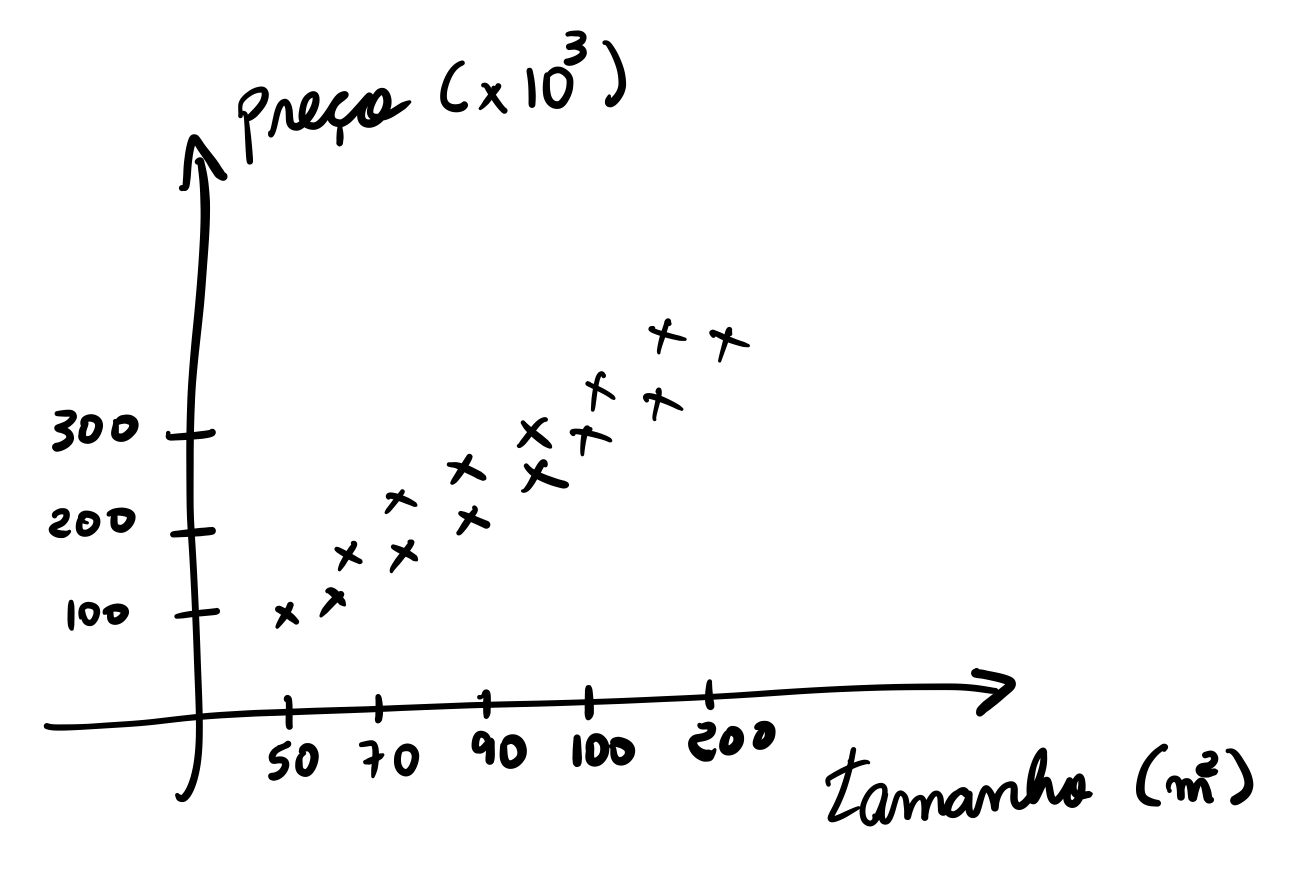
\includegraphics[scale=0.1]{./figs/Regressao_Linear_Fig1.png}
\onslide<3->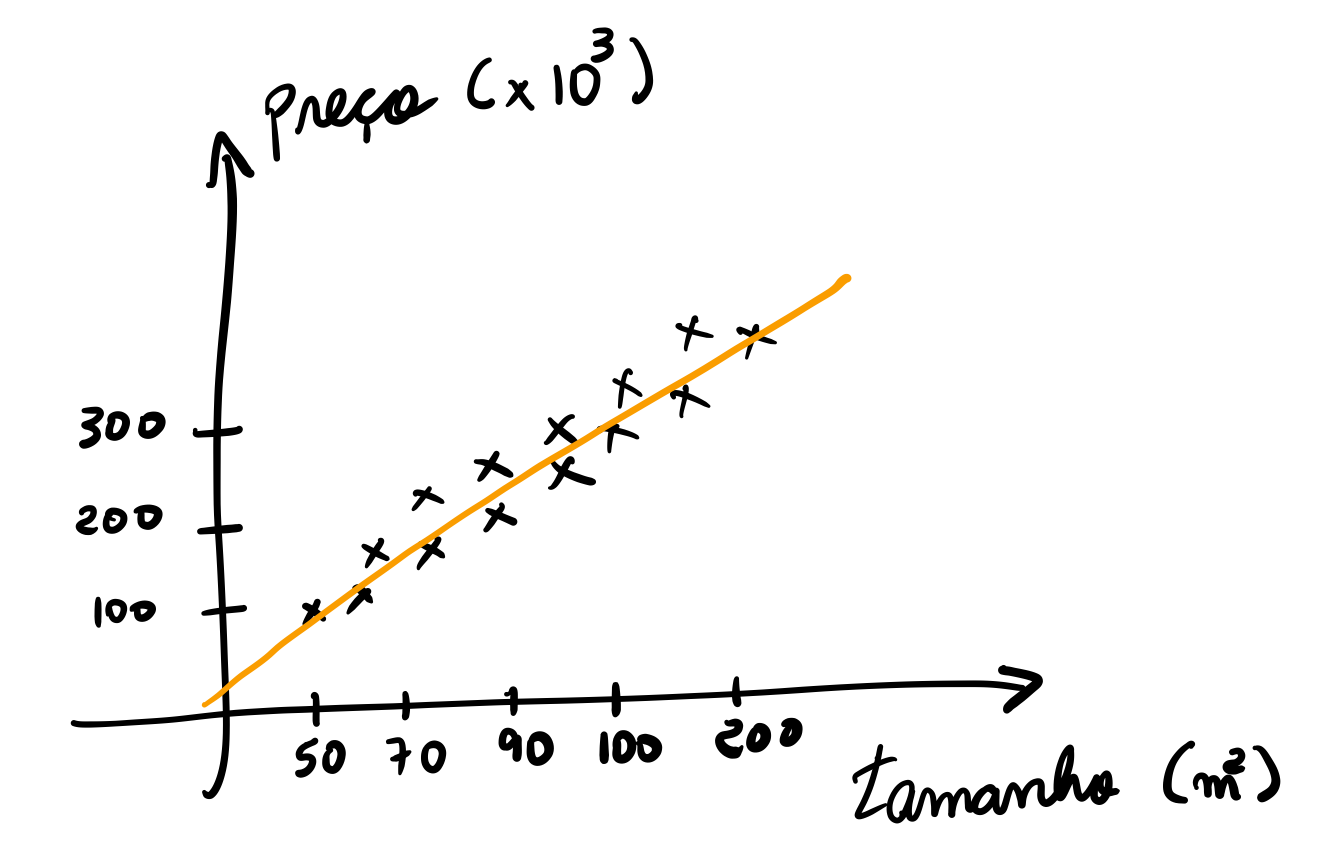
\includegraphics[scale=0.1]{./figs/Regressao_Linear_Fig2.png}
\end{center}

%\secxx{Sub-Section}

% EXERCISE
%\exe{4}{Exercise}
% SUGGESTED READING BOX			
%\sug{References}
% CITATION						
%\cittex{Citation}

}%%%%%%%%%%%%%%%%%%%%%%%%%%%%%%%%%%%%%%%%%%%%%%%%%%
% ###############################################################################
% SLIDE NO TITLE
\Sli{
\justify \underline{Definição do problema:} seja um conjunto de dados ${\cal X}= \{(x_1,y_1),(x_2,y_2),\ldots,(x_z,y_z)\}$ tal que $x_i\in\mathbb{R}$ corresponde ao dado de entrada e $y_i\in\mathbb{R}$ denota o seu respectivo valor de saída. Temos, ainda, que ${\cal X}$ pode ser \textbf{particionado} da seguinte forma: ${\cal X} = {\cal X}^1\cup {\cal X}^2$, em que ${\cal X}^1$ e ${\cal X}^2$ denotam os conjuntos de dados de \textbf{treinamento} e \textbf{teste}, respectivamente. Nosso objetivo é, dado o conjunto de treinamento, aprender uma função $h:\mathbb{R}\rightarrow\mathbb{R}$ que consiga estimar o valor de uma casa dado o seu tamanho.

\begin{center}
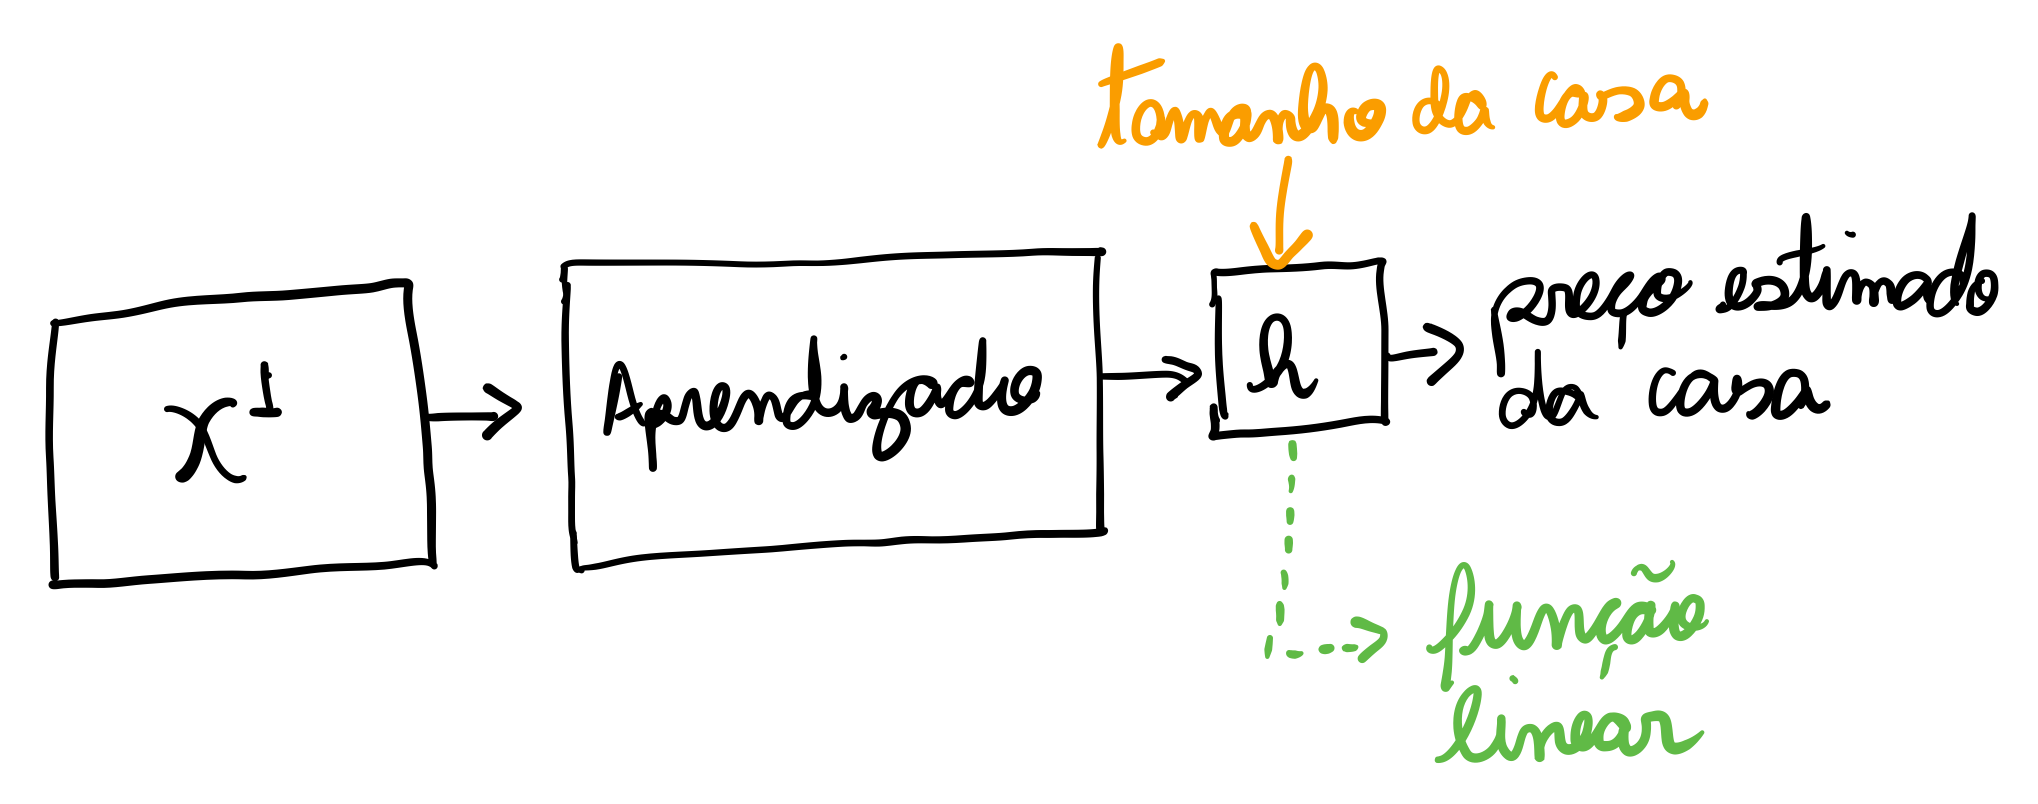
\includegraphics[scale=0.1]{./figs/Regressao_Linear_Fig3.png}
\end{center}
}

\Sli{
\justify A técnica chama-se \textbf{Regressão Linear Univariada} porque aprendemos uma \textbf{função linear} utilizando apenas \textbf{uma} variável de entrada. Desta forma, temos a seguinte formulação para essa função:

\begin{equation}
\label{e.hx}
	h_{\boldsymbol{w}}(x)=w_0+w_1x,
\end{equation}
em que $w_0$ e $w_1$ denotam os parâmetros do modelo (equação da reta), podendo ser representados como $\boldsymbol{w}=[w_0\ w_1]$.
\begin{center}
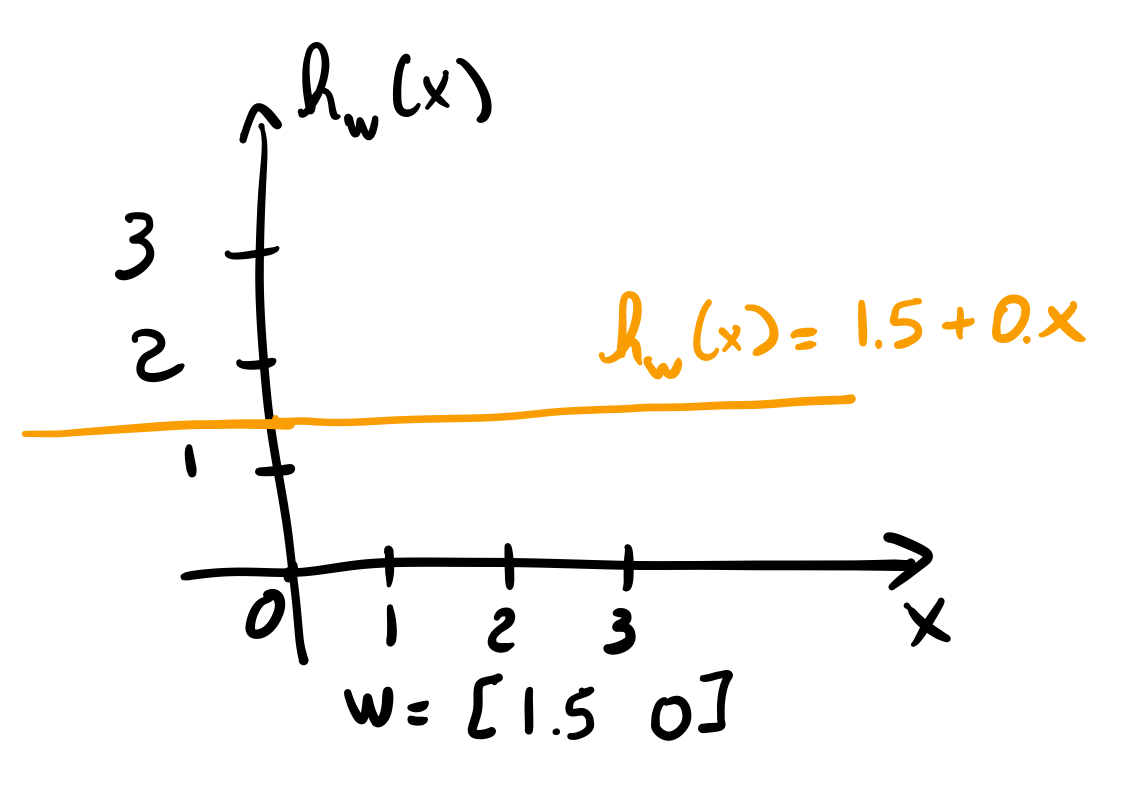
\includegraphics[scale=0.1]{./figs/Regressao_Linear_Fig4.png}\hspace{1cm}
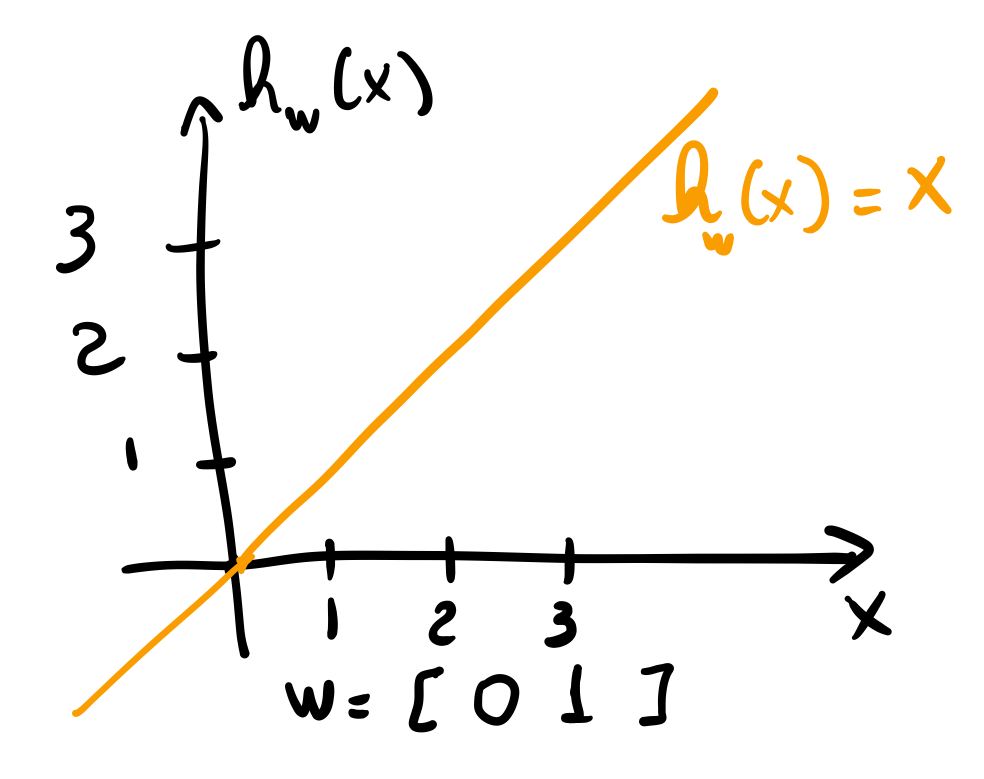
\includegraphics[scale=0.1]{./figs/Regressao_Linear_Fig5.png}\hspace{1cm}
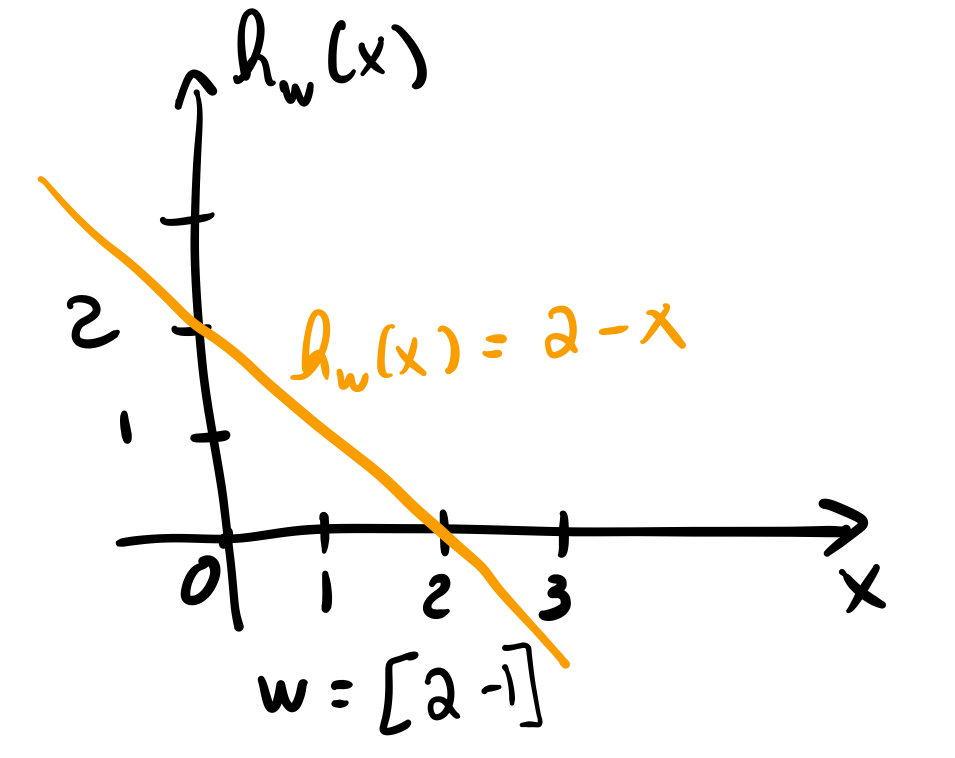
\includegraphics[scale=0.1]{./figs/Regressao_Linear_Fig6.png}
\end{center}

}%%%%%%%%%%%%%%%%%%%%%%%%%%%%%%%%%%%%%%%%%%%%%%%%%%

\Sli{
\justify Desta forma, como podemos observar, temos diferentes comportamentos para $h_{\boldsymbol{w}}(x)$, a qual é também chamada de \textbf{função hipótese}. A ideia principal da regressão linear é escolher o vetor de parâmetros $\boldsymbol{w}$ tal que $h_{\boldsymbol{w}}(x)$ seja a mais próxima possível das saídas das amostras de nosso conjunto de treinamento. Matematicamente falando, temos o seguinte problema de \textbf{minimização}:

\begin{equation}
\label{e.min_linear_regression}
	\boldsymbol{w}^\ast = \argmin_{\boldsymbol{w}}\left\{\frac{1}{2m}\sum_{i=1}^m(h_w(x_i)-y_i)^2\right\},
\end{equation}
em que $m$ denota o tamanho do conjunto de treinamento.
}

\Sli{
A Equação 2 é usualmente chamada de \textbf{função de custo}, também conhecida por \textbf{erro médio quadrático}. Podemos simplificar a notação escrevendo a Equação 2 da seguinte forma:

\begin{equation}
\label{e.min_linear_regression_simplified}
	\boldsymbol{w}^\ast = \argmin_{\boldsymbol{w}}\{J(\boldsymbol{w})\},
\end{equation}
em que 

\begin{equation}
\label{e.cost_function}
J(\boldsymbol{w}) = \frac{1}{2m}\sum_{i=1}^m(h_w(x_i)-y_i)^2. 
\end{equation}
No entanto, vamos simplificar um pouco mais o problema e assumir que $\boldsymbol{w} = [0\ w_1]$, ou seja, vamos assumir que $w_0 = 0$ (a reta passa na origem do sistema de coordenadas).
}

\Sli{
Assim sendo, a Equação 1 pode ser escrita da seguinte forma:

\begin{equation}
	h_{\boldsymbol{w}}(x)  = w_0 +w_1x = w_1x.
\end{equation}

\begin{center}
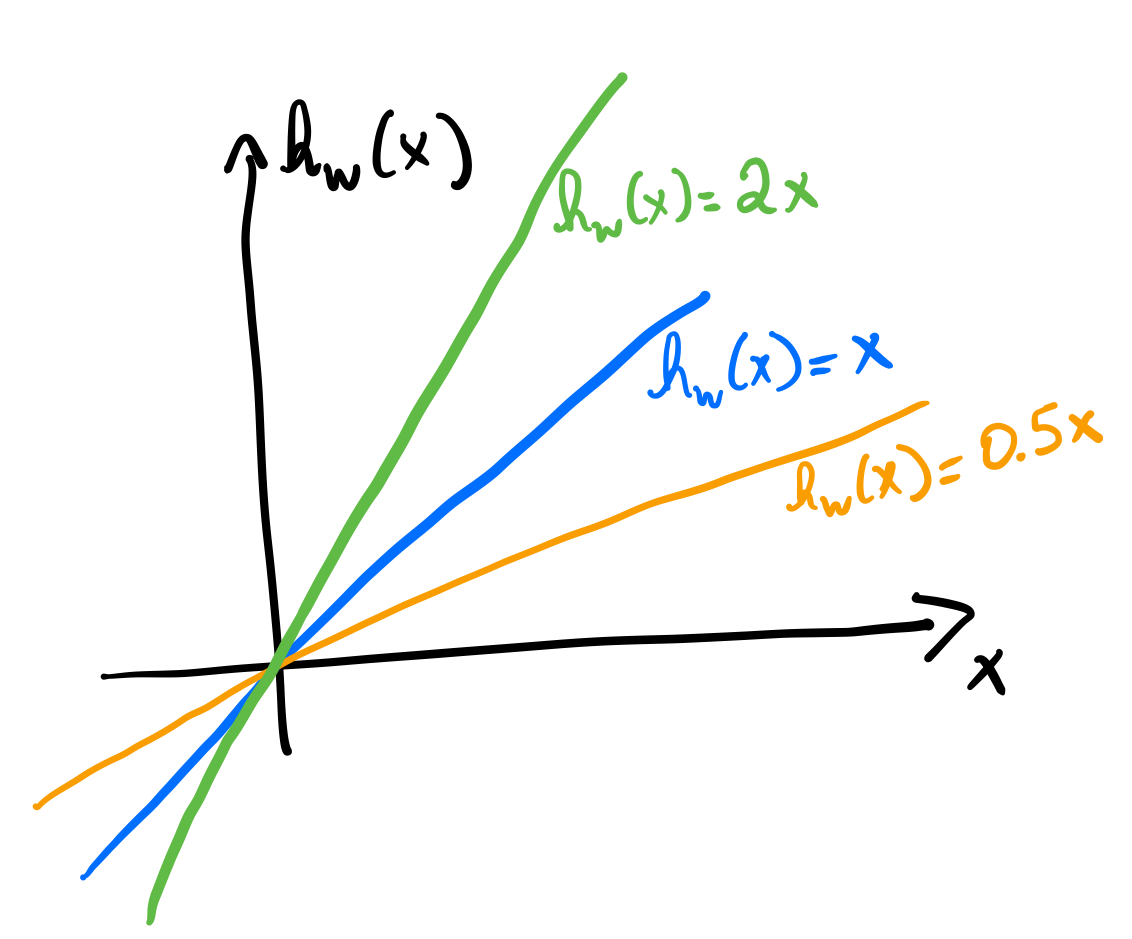
\includegraphics[scale=0.13]{./figs/Regressao_Linear_Fig7.png}\hspace{1cm}
\end{center}
}

\Sli{
Assumindo, então, que $w_0=0$, podemos escrever a Equação 3 da seguinte forma:

\begin{equation}
\label{e.min_linear_regression_simplified}
	\boldsymbol{w}^\ast = \argmin_{w_1}\left\{J(w_1)\right\}.
\end{equation}
\justify O nosso problema passar a ser, agora, encontrar um valor apropriado para $w_1$ de tal forma que o valor de $J(w_1)$ seja o menor possível. Resumindo, o que temos definido até então para o problema:

\begin{itemize}
	\item Função hipótese: $h_{\boldsymbol{w}}(x)$
	\item Função de custo: $J(\boldsymbol{w})\approx J(w_1)$
\end{itemize}
}	

\end{document}